\documentclass[12pt]{article}
\usepackage[T1]{fontenc}
\usepackage[utf8]{inputenc}
\usepackage{url}
\usepackage{enumerate}
\usepackage[top=3cm, bottom=3cm]{geometry}
\usepackage{graphicx}
% \usepackage{enumitem}
\usepackage{natbib}
\usepackage{listings}
\usepackage{float}
\usepackage{amsmath}
\usepackage{color}
\bibpunct{[}{]}{,}{a}{}{;}
\setcitestyle{super}

% Variables
\newcommand{\assignmentname}{Assignment 1}
\newcommand{\coursename}{Advanced Algorithms and Data Structures}
\newcommand{\studentname}{Bjarki Madsen (lch929) - Michael Bang (tqg432)}
\newcommand{\department}{Department of Computer Science}
\newcommand{\institution}{Copenhagen University}
\newcommand{\location}{Copenhagen, Denmark}

\begin{document}

\renewcommand\refname{References}

\title{\assignmentname \\ {\Large {\textsc \coursename}}}
\author{
        \studentname \\
        \department \\
        \institution \\
        \location
}
\date{\today}

\maketitle
\thispagestyle{empty}

\pagebreak

\section*{Exercise 1}

  Figure \ref{fig:e1_a_solution} shows a b-flow with flow value of 9 for the first proposed graph from the assignment. The second proposed graph has no b-flow. The reason is that $v_1$ wants to have at least $3 + c(v_2, v_1)$ after giving away $f(v_1, v_3)$. In order for that to happen the $f(v_2, v_1)$ has to equal to $c(v_2, v_1)$. After the $f(v_2, v_1)$, $v_2$ wants to end up with 1 in demand, meaning it needs a flow value of 4 to itself but that is impossible because the maximum flow to $v_2$ is equal to $c(v_3, v_2)$, or 2 and therefore is unable to fulfill $f(v_2, v_1) = c(v_2, v_1)$.

  \begin{figure}[h]
    \centering
      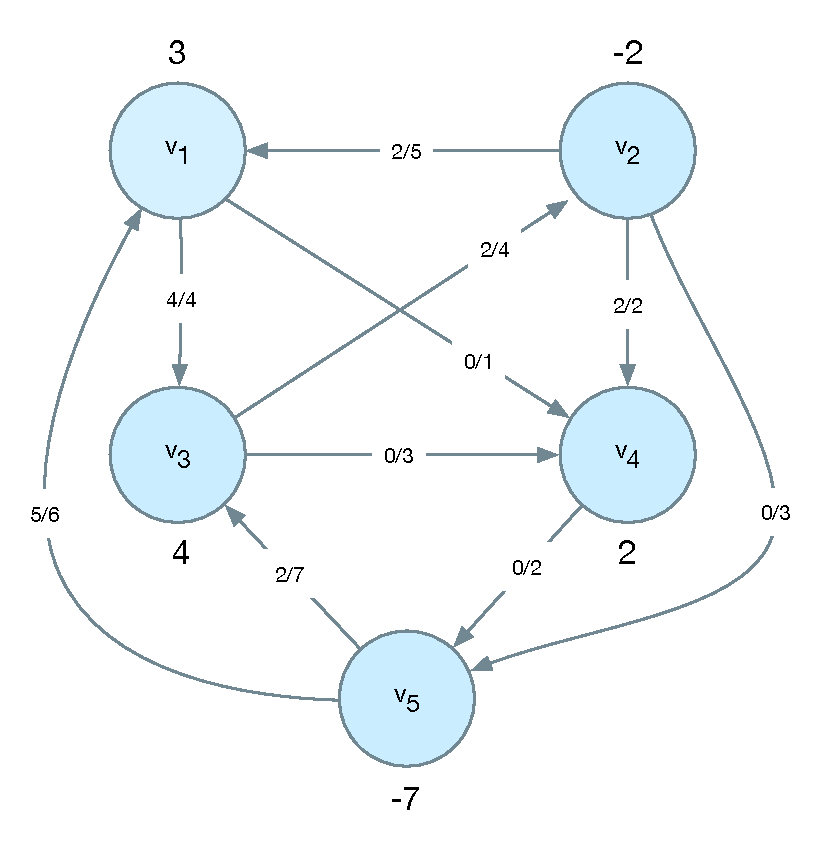
\includegraphics[width=0.6\textwidth]{figures/e1_a_solution}
    \caption{Graph showing b-flow with flow value 9}
    \label{fig:e1_a_solution}
  \end{figure}

\section*{Exercise 2}
\subsection*{Exercise 2.1}

  Tables \ref{table:values_xvf} and \ref{table:values_zfg} show the values for $x_{vf}$ and $z_{fg}$, respectively. The number of breakpoints are 13. Figure \ref{fig:e2_1} shows the rectilinear layout based on the planar embedding given in the assignment description.

  \begin{table}[h]
    \centering
    \begin{tabular}{llllllll}
                                    & \textbf{v1} & \textbf{v2} & \textbf{v3} & \textbf{v4} & \textbf{v5} & \textbf{v6} & \textbf{v7} \\ \cline{2-8}
    \multicolumn{1}{c|}{\textbf{a}} & 0           & 0           & 1           & 0           & 1           & 1           & 0           \\
    \multicolumn{1}{l|}{\textbf{b}} & 1           & 0           & 0           & 0           & 0           & 1           & 0           \\
    \multicolumn{1}{l|}{\textbf{c}} & 1           & 1           & 1           & 0           & 0           & 0           & 0           \\
    \multicolumn{1}{l|}{\textbf{d}} & 0           & 1           & 1           & -1          & 0           & 1           & 0           \\
    \multicolumn{1}{l|}{\textbf{e}} & 0           & 0           & 1           & 1           & -1          & 1           & 0
    \end{tabular}
    \caption{The values for $x_{vf}$. For example, $v_1$ has inner turn in the boundary cycle $b$.}
    \label{table:values_xvf}
  \end{table}

  \begin{table}[h]
    \centering
    \begin{tabular}{llllll}
                                    & \textbf{a} & \textbf{b} & \textbf{c} & \textbf{d} & \textbf{e} \\ \cline{2-6}
    \multicolumn{1}{l|}{\textbf{a}} & 0          & 2          & 1          & 0          & 4          \\
    \multicolumn{1}{l|}{\textbf{b}} & 0          & 0          & 1          & 1          & 0          \\
    \multicolumn{1}{l|}{\textbf{c}} & 0          & 1          & 0          & 0          & 0          \\
    \multicolumn{1}{l|}{\textbf{d}} & 0          & 1          & 0          & 0          & 0          \\
    \multicolumn{1}{l|}{\textbf{e}} & 0          & 0          & 0          & 2          & 0
    \end{tabular}
    \caption{The values for $z_{fg}$. For example, the number of inner turns in the breakpoints of the edges that $d$ shares with $b$ is 2.}
    \label{table:values_zfg}
  \end{table}

  \begin{figure}[h]
    \centering
      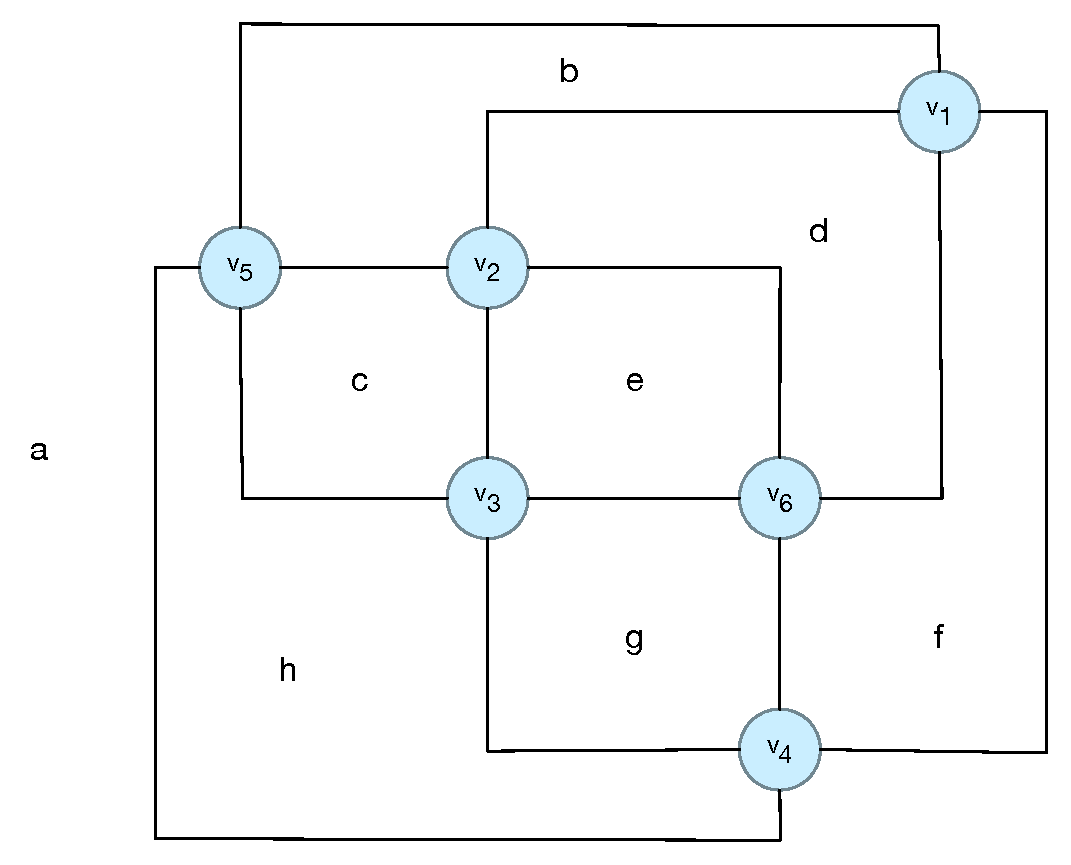
\includegraphics[width=0.6\textwidth]{figures/e2_1}
    \caption{A rectilinear layout based on the planar embedding in Figure 2(b) from the assignment description.}
    \label{fig:e2_1}
  \end{figure}


\subsection*{Exercise 2.2}

  The sum of all the turns that $f$ makes in its vertices is:
  $$\sum_{f \in F, v \in V}{x_{vf}}$$
  The sum of all the inner turns that $f$ makes in its breakpoints is:
  $$\sum_{f \in F}\sum_{g \in F \setminus f}z_{fg}$$
  If there exists an inner turn from $g$ to $f$, it must mean that that turn is an outer turn seen from $f$ to $g$ so we can therefore sum the outer turns up as following:
  $$\sum_{f \in F}\sum_{g \in F \setminus f}z_{gf}$$
  which can be combined to a single sum:
  $$\sum_{f \in F}\sum_{g \in F \setminus f}(z_{fg} - z_{gf})$$
  We then combine these equations and state them as the following constraints:
  \begin{align*}
      \sum_{f \in F, v \in V}(x_{vf}) + \sum_{f \in F}\sum_{g \in F \setminus f}(z_{fg} - z_{gf}) = \begin{cases}
                                                                                       4, & \text{if } f \text{ is internal}\\
                                                                                      -4, & \text{otherwise}
                                                                                   \end{cases}
  \end{align*}

  Finally, let's verify that the constraints hold for faces $a$ and $e$ from Figure 3 in the assignment description. We look up the values in Table \ref{table:values_xvf} and \ref{table:values_zfg}:
  \begin{align*}
    a &: x_{v_{3}a} + x_{v_{5}a} + x_{v_{6}a} + ((z_{ab} - z_{ba}) + (z_{ac} - z_{ca}) + (z_{ae} - z_{ea}))\\
      &= 1 + 1 + 1 + ((0 - 2) + (0 - 1) + (0 - 4)) \\
      &= -4
  \end{align*}
  \begin{align*}
    e &: x_{v_{3}e} + x_{v_{4}e} - x_{v_{5}e} + x_{v_{6}e} + ((z_{ea} - z_{ae}) + (z_{ed} - z_{de}))\\
      &= 1 + 1 -1 + 1 + ((4 - 0) + (0 - 2)) \\
      &= 4
  \end{align*}

\subsection*{Exercise 2.3}
It is a necessary but not sufficient condition for $G$ to be a rectilinear layout that no vertex has degree greater than 4. We see that this is the case by looking at the different ways in which we can connect edges to a vertex. Given the constraints that edges mustn't cross, and that they must be either vertical or horizontal, we find that there are only four ways to connect an edge to a vertex, namely the four cardinal directions.\\
\\
The restrictions on edges already mentioned also mean there are at most four different ways in which we can connect between two and four edges to a vertex, considering rotation of the vertex and edges not to have any meaning. These four ways to connect edges are shown on Figure \ref{fig:e1_a_solution}.

\begin{figure}[h]
    \centering
      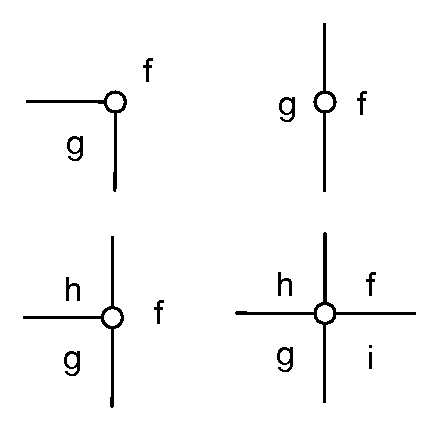
\includegraphics[width=0.4\textwidth]{figures/e2_3}
    \caption{The four different ways to connect edges to a vertex, given the vertical/horizontal and non-crossing edges constraints.}
    \label{fig:e2_3}
\end{figure}

\subsection*{Exercise 2.4}

  Based on the previously stated variables, we can now count the total number of breakpoints in the rectilinear layout as the following:
  $$\sum_{f \in F}\sum_{g \in F \setminus f} z_{fg}$$
  where $z_{fg}$ is the number of inner turns in the breakpoints between $f$ and $g$. We need not worry about not counting any outer turns since those will be counted as inner turns when we look at $z_{gf}$.

  Our objective function therefore becomes:
  \begin{equation*}
    \begin{aligned}
    & {\text{minimize}}
    & & \sum_{f \in F}\sum_{g \in F \setminus f} z_{fg} \\
    & \text{subject to}
    & & \sum_{f \in F, v \in V}(x_{vf}) + \sum_{f \in F}\sum_{g \in F \setminus f}(z_{fg} - z_{gf}) = \begin{cases}
                                                                                      4, & \text{if } f \text{ is internal}\\
                                                                                      -4, & \text{otherwise}
                                                                                     \end{cases} \\
    & & &  \sum_{f \in F}{x_{vf}} = \begin{cases}
                                        0 & \text{if v has degree 2}\\
                                        2 & \text{if v has degree 3}\\
                                        4 & \text{if v has degree 4}
                                    \end{cases}\\
    & & & z_{fg} \geq 0
    \end{aligned}
  \end{equation*}

\subsection*{Exercise 2.5}

We have:

\begin{align*}
      \sum_{f \in F, v \in V}(x_{vf}) + \sum_{f \in F}\sum_{g \in F \setminus f}(z_{fg} - z_{gf}) = \begin{cases}
                                                                                       4, & \text{if } f \text{ is internal}\\
                                                                                      -4, & \text{otherwise}
                                                                                   \end{cases}
\end{align*}
Making the following substitution for $x_{vf}$ :
\begin{align*}
  x_{vf} =  \begin{cases}
               1, & \text{if } f \text{ makes an inner turn in } v \\
               0, & \text{otherwise.}
            \end{cases}
\end{align*}
we can write:

\begin{align*}
  \sum_{f \in F, v \in V}{x_{vf}^{-}} - \sum_{f \in F, v \in V}{x_{vf}^{+}} + \sum_{f \in F}\sum_{g \in F \setminus f}(z_{fg} - z_{gf}) = \begin{cases}
                                                                                       4, & \text{if } f \text{ is internal}\\
                                                                                      -4, & \text{otherwise}
                                                                                   \end{cases}
\end{align*}
where $x_{vf}^{-}$ represents an inner turn and $x_{vf}^{+}$ represents an outer turn.

We then rewrite: (TODO fix alignment problem)
\begin{align*}
  &= \sum_{f \in F, v \in V}{x_{vf}^{-}} - \sum_{f \in F, v \in V}{x_{vf}^{+}} + \sum_{f \in F}\sum_{g \in F \setminus f}(z_{fg} - z_{gf})\\
  &= \sum_{f \in F, v \in V}{x_{vf}^{-}} - \sum_{f \in F, v \in V}{x_{vf}^{+}} + \sum_{f \in F, g \in F\setminus f}{z_{fg}} - \sum_{f \in F, g \in F \setminus f}z_{gf}\\
  &= \sum_{f \in F, v \in V}{x_{vf}^{-}} + \sum_{f \in F, g \in F\setminus f}{z_{fg}} - \sum_{f \in F, v \in V}{x_{vf}^{+}} - \sum_{f \in F, g \in F \setminus f}z_{gf}\\
\end{align*}~\\
The first two terms of the last equation above represent inner turns, while the two latter terms represent outer turns. We rename these pairs of terms to $y_e$ where $e$ is an edge
\begin{align*}
  &= \sum_{e \in \delta^{-}(v)}{y_e} - \sum_{e \in \delta^{+}(v)}{y_e} = b_v, \forall v \in V = b, \forall{e} \in E
\end{align*}

where $\delta^{-}(v)$ represents the set of inner turns in the original vertices and breakpoints and $v$ is a vertix in the flow-graph, and $\delta^{+}(v)$ represents the same, but for outer turns.


The vertices in the MCFP graph will consist of the faces \textit{and} the original vertices of the planar embedding. The edges in the flow graph will be between:

\begin{enumerate}[(i)]
  \item faces which are adjacent in the planar embedding
  \item vertices in the planar embedding which lie on a boundary cycle of a face
\end{enumerate}

The demand for a vertex $v$ if the vertex represents a face in the planar embedding is given by the formula:

\begin{align*}
    demand(v) = \begin{cases}
                  4  & \text{if } v \text{ represents a internal face}\\
                  -4 & \text{if } v \text{ represents a external face}
                \end{cases}
\end{align*}

The demand for a vertex $v$ if $v$ represents an original vertex in the planar embedding is given by the formula:
\begin{align*}
    demand(v) = \begin{cases}
                  0  & \text{if } v \text{ has degree 2} \\
                  -2 & \text{if } v \text{ has degree 3} \\
                  -4 & \text{if } v \text{ has degree 4}
                \end{cases}
\end{align*}

The capacities between faces which share an edge in the flow graph are unbounded with a cost of 1. The reason why they are unbounded is because we can have unlimited number of breakpoints between faces. The capacity of edges starting in an original vertex is 1 because it can provide at most 1 inner turn to a face. The cost on these edges is none since there is a vertex lying on these kind of breakpoints.

Figure \ref{fig:mcfp_instance} shows an instance of a MCFP for the original planar embedding shown in figure \ref{fig:planar_embedding}. The edges painted in red have cost equal to 1 and the black edges have cost equal to 0. The flow across a red edge represents the number of breakpoints between adjacent faces in the rectilinear layout. Flow across a black edge represents a vertex $v$ making an inner turn in a face $f$.

\begin{figure}[h]
  \centering
    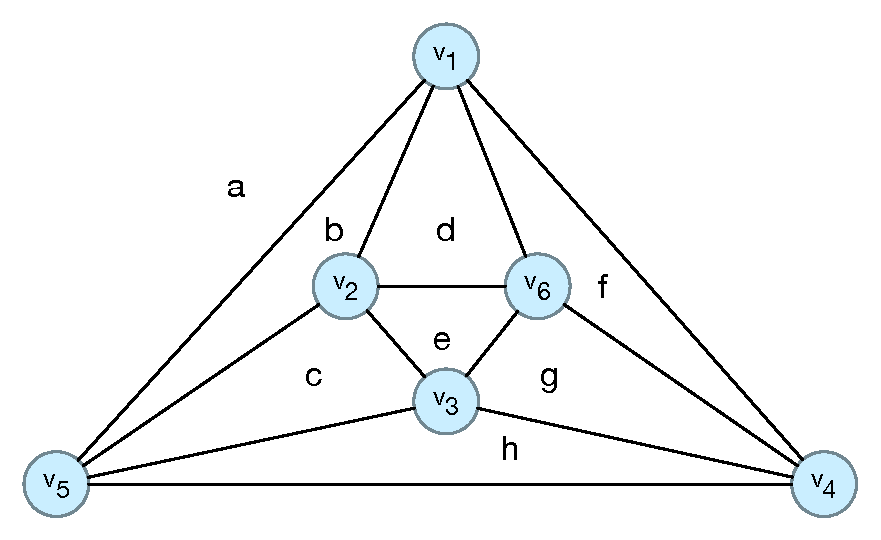
\includegraphics[width=0.6\textwidth]{figures/e2_5_planar_embedding}
  \caption{The original planar embedding.}
  \label{fig:planar_embedding}
\end{figure}

\begin{figure}[h]
  \centering
    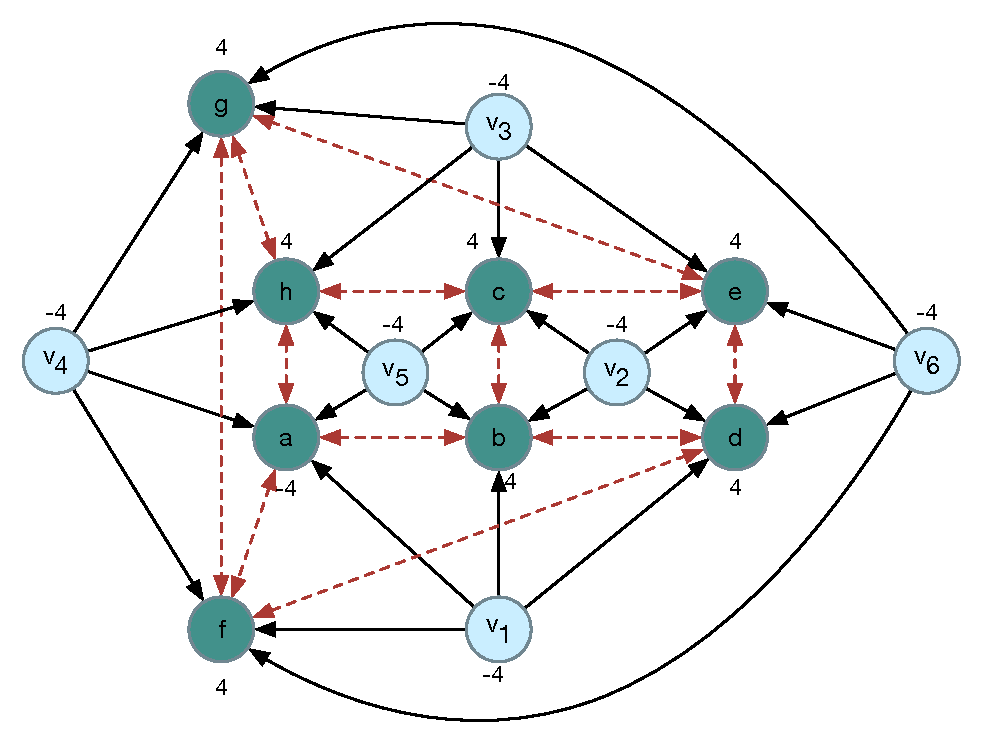
\includegraphics[width=0.8\textwidth]{figures/e2_5}
  \caption{An instance of MCFP corresponding to the embedded graph in Figure \ref{fig:planar_embedding}.}
  \label{fig:mcfp_instance}
\end{figure}

\section*{3}
\subsection*{3.1}
We have identified four different cases which we need to consider for this task:
\begin{enumerate}
    \item $l_e$ and $u_e$ are both finite
    \item $l_e$ is finite, $u_e$ is $\infty$
    \item $l_e$ is $-\infty$, $u_e$ is finite
    \item $l_e$ is $-\infty$ $u_e$ is $\infty$
\end{enumerate}~\\
\\
The first three cases are trivial; it's clear that at least one of the variables is finite. The fourth case is interesting, though. We found that we can perform a transformation of the vertices such that at least one of the variables is finite. This is shown on Figure \ref{fig:e3_1}.

\begin{figure}[h]
  \centering
    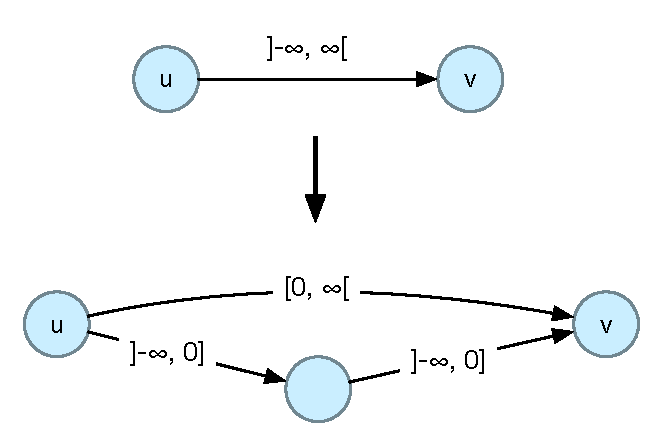
\includegraphics[width=0.6\textwidth]{figures/e3_1}
  \caption{Transformation of case 4, ensuring that at least one of $l_e$ and $u_e$ is finite.}
    \label{fig:e3_1}
\end{figure}~\\
\\
In the transformation we split the capacity over two edges instead of one, meaning that at least one of the variables is finite for each edge. It's clear that we maintain the same overall capacity between the edges, because the union of the two new ranges is equal to the original range.\\
\\
We see that our transformation adds one vertex and two edges per edge which has a capacity of $]-\infty;\infty[$. This means that in the worst case, we will add at most $2\cdot E$ edges and $E$ vertices, both of which are constant w.r.t. the original graph.\\
\\
We now know how to transform $I_0$ to $I_1$ where at least one of the variables $l_e$ and $u_e$ are finite on each edge.

\subsection*{3.2}
Looking at the four cases listed in Section 3.1 we see that two of them are trivial, and that we need only focus our attention to the other two, namely cases 3 and 4.\\
\\
We will first consider case 4. From the result in Section 3.1 we know how to transform case 4 to the figure shown on Figure \ref{fig:e3_1}. Once we've applied this transformation, we can begin looking at the meaning of having a negative capacity. Having a negative capacity over an edge $(v_1, v_2)$ is the same as having a positive capacity over the edge $(v_2, v_1)$. We can see this by lookig at the equation given in the assignment
\begin{align*}
    \sum_{e\in \delta^-(v)}{x_e}-\sum_{e\in \delta^+(v)}{x_e} = b_v, \forall{v} \in V
\end{align*}~\\
\\
Writing out the formula for the specific case of $v_1$ in Figure \ref{fig:e3_2_b} we get the following (note that the operational sign of $e_2$ changes on the right side of the equation because the direction of the edge is changed.)
\begin{align*}
    \sum_{e\in \emptyset}{x_e} - \sum_{e\in \{e_1, e_2\}}{x_e} =
    \sum_{e\in \{-e_2\}}{x_e} - \sum_{e\in \{e_1\}}{x_e} = b
\end{align*}~\\
\\
Figure \ref{fig:e3_2} shows the transformation we make in case 4 (where the transformation from Section 3.1 has already been applied.)

\begin{figure}[h]
  \centering
    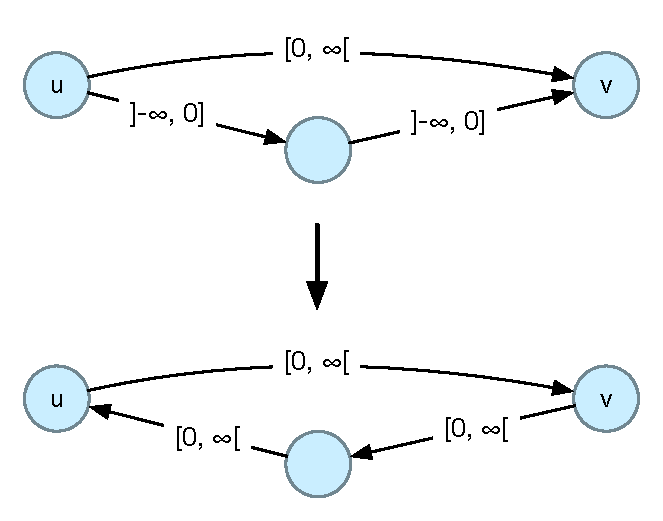
\includegraphics[width=0.6\textwidth]{figures/e3_2}
  \caption{Transformation of case 4, ensuring that $l_e$ is finite}
  \label{fig:e3_2}
\end{figure}

\begin{figure}[h]
  \centering
    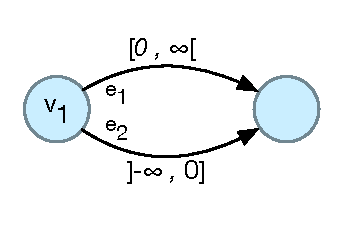
\includegraphics[width=0.4\textwidth]{figures/e3_2_b}
  \caption{Vertex which has edges of both positive and negative capacity}
  \label{fig:e3_2_b}
\end{figure}~\\
\\
We now consider case 3. From what we just showed above, it is clear that we can use the same approach; the edge $(v_1, v_2)$ with negative capacity is the same as having the edge $(v_2, v_1)$ with a positive capacity. Since $u_e$ is finite in this case, we know that $l_e$ will be so after the transformation.\\
\\
We now know how to transform $I_1$ to $I_2$ such that $l_e$ is finite.

\subsection*{3.3}
From the previous sections we know how to transform the graph such that $l_e$ is finite. We now show how we can further transform it such that $l_e  = 0$.\\
\\
In this transformation we add a node $x$ on the edge $(u, v)$ as shown on Figure \ref{fig:e3_3}, where we know that $l_e$ is finite. The new vertex has a demand of $l_e$, ensuring that at least $l_e$ flows over the new edge added, even after the capacity of the edge $(u, x)$ has been set to 0.\\
This transformation adds one edge and one vetex to the graph. This means that, in the worse case, we will add at most $E$ edges and $E$ vertices to the graph, both of which are constant w.r.t. the original graph.\\
\\
Combining what we showed in Sections 3.1, 3.2, and 3.3, we can now transform instances of GMCFP graphs to instances of MCFP graphs.

\begin{figure}[h]
  \centering
    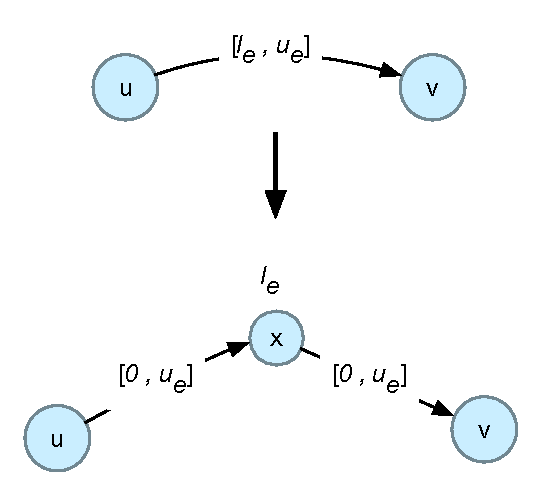
\includegraphics[width=0.6\textwidth]{figures/e3_3}
  \caption{Transformation of finite $l_e$ ensuring that $l_e$ is equal to 0 while maintaining the required flow on the edges.}
  \label{fig:e3_3}
\end{figure}

\subsection*{3.4}
Only the transformations in Sections 3.1 and 3.3 add edges and vertices to the graph.\\
In Section 3.1 we saw that in the worst case we would add at most $2E$ edges and $E$ vertices. In Section 3.3 we saw that we would add at most $E$ edges and $E$ vertices.\\
We see that the worst case for Section 3.1 and 3.3 can't happen at the same time; the transformations from Section 3.1 and 3.2 can always be applied in succession, which will leave $l_e = 0$ for all edges where these transformations were used. The transformation in Section 3.3 requires that $l_e \ne 0$, and thus can't be used after transformation 3.2. This means that we will at most add a constant number of edges and vertices, and will be within the bound of $O(V+E)$ edges and vertices.

\end{document}
% End of document.

